\chapter{Evaluation}
\label{ch:evaluation}

\section{Empirical Data}

\subsection{Performance}

We tested the existing ui5 implementation and the new SvelteKit Implementations, in multiple metrics. We were especially interested in responsiveness to navigation events. To this end we measured first contentful paint (FCP), the time until the page settled, and cumulative layout shift (CLS). Furthermore, we measured time until the page settled, for a navigation from the chauffeur job overview, to the details view of a chauffeur job.

All measurements were conducted on a Lenovo ThinkPad T480, with an Intel Core i7-8550U, and 16 GB RAM, running Windows 11. The measurements where taken using the developer tools of Google Chrome 116.0. The benchmark setup is described in app. \ref{app:benchmark-setup}.

Our measurements (fig. \ref{fig:benchmark}) show, while our implementations took longer to send content to the client, they reduced time until the relevant data is being shown, significantly. These results align with the expected effects of server side rendering, outlined in section \ref{sec:rendering-patterns}. Furthermore, SvelteKit shows significant improvements when navigating between two pages. This is improved even further by SvelteKit's preloading capabilities. In our benchmark, preloading was set to "tap", meaning, the data is being fetched as soon as a \mintinline{html}|mousedown| event is triggered. This data is shown in Pdown nav. While Pup nav shows the time from, when a click event is fired.  

\begin{figure}
    \centering
    \begin{tikzpicture}
        \begin{axis}[
                ybar,
                bar width=.7cm,
                width=\textwidth,
                height=.5\textwidth,
                legend style={at={(0,1)},
                    anchor=north west,legend columns=1},
                legend cell align={left},
                symbolic x coords={TTFB,FCP,CP,Nav},
                xtick=data,
                enlarge x limits={0.15},
                nodes near coords,
                nodes near coords align={vertical},
                ymin=0,ymax=4000,
                ylabel={duration (ms)},
            ]
            \addplot table[x=type,y=ui5]{\benchmarkdata};
            \addplot table[x=type,y=sk-fs]{\benchmarkdata};
            \addplot table[x=type,y=sk-fe]{\benchmarkdata};
            \legend{UI5, SvelteKit Full Stack, SveleKit FE-only}
        \end{axis}
    \end{tikzpicture}
    \label{fig:benchmark}
    \caption{Benchmark Results for TTFB, FCP, CP and Nav}
\end{figure}

Levlin, has shown, that SvelteKit can provide significant improvements in certain areas over frameworks like react and angular.  

\subsection{Bundle Size}

Smaller, but no data yet... fuck all 

\subsection{Something else}

% \begin{itemize}
%     \item SEO
%     \item Community support
%     \item DX
%     \item ecosystem
%     \item performance
% \end{itemize}

\section{Experience}

% \begin{itemize}
%     \item Both approaches (full stack and frontend only) worked great
%     \item advantage of full-stack: 
%     \item no API definition required
%     \item reuse of models between UI and business logic or even type inference
% \end{itemize}

In this section we give our personal experience developing with SvelteKit in an attempt to reason about SvelteKit's expected developer experience. As we noted before, providing a heuristic analysis of SvelteKit's DX is out of scope.

In our experience both discussed implementations (full stack in SvelteKit and SvelteKit only for frontend) enabled an efficient and pleasant development experience. Especially the full stack approach significantly reduced overhead, because models could be reused between client and server and communication between server and client happened transparently.

% \begin{itemize}
%     \item Concise / Intuitive Syntax
%     \item reduction of client-server waterfalls
%     \item SPA/SSR/SSG with single framework
%     \item clear data flow (load function $\rightarrow$ svelte, svelte $\rightarrow$ action)
% \end{itemize}

% todo: reactivity pitfalls (e.g. dependencies in functions)

\subsection{Project Setup}

\Cref{fig:project-setup}

% \begin{itemize}
%     \item Fast, \mintinline{bash}|npm cgeate svelte@latest|
%     \item missing out-of-the-box features: form validation/parsing
% \end{itemize}



\begin{figure}
    \centering
    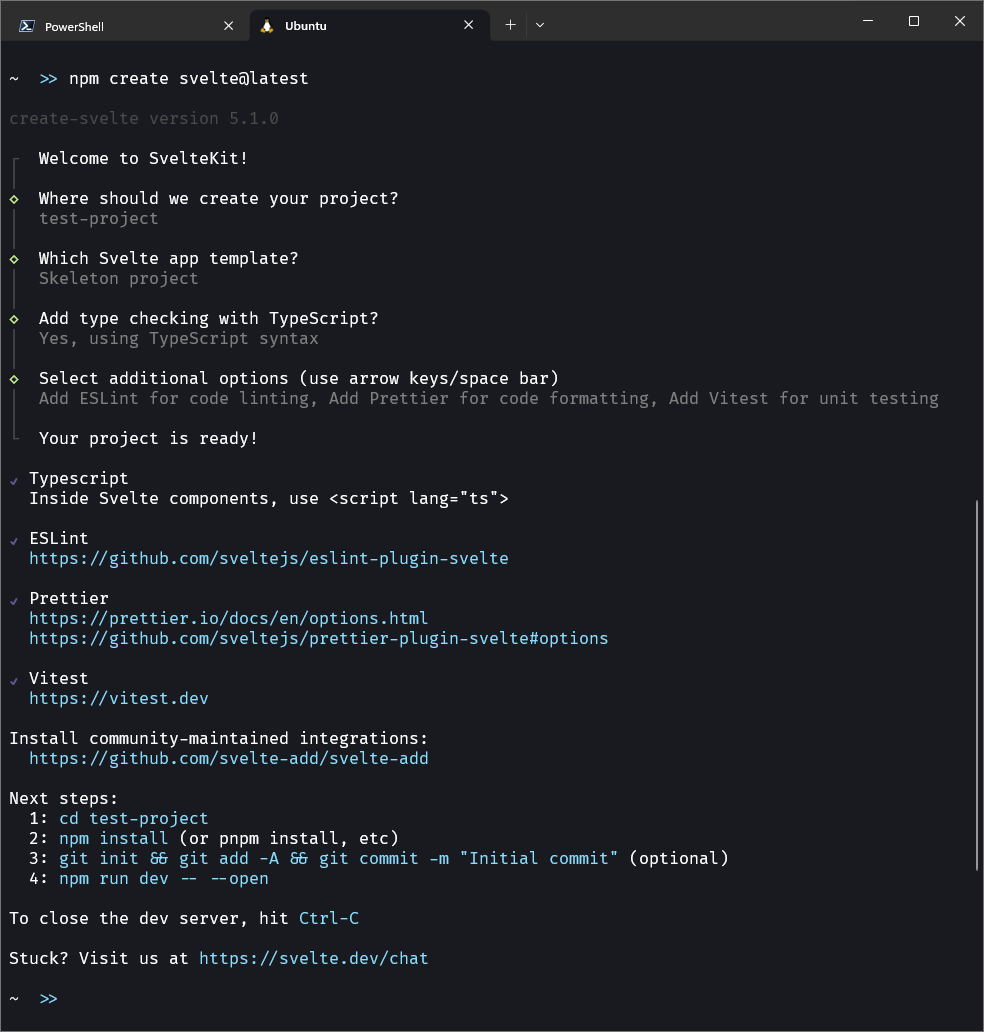
\includegraphics[width=\linewidth,trim={0 15cm 0 1.5cm},clip]{assets/sveltekit-project-setup}
    \caption{Process for creating a new SvelteKit project}
    \label{fig:project-setup}
\end{figure}

\subsection{Syntax}

We experienced Svelte's syntax as easy to grasp. This is because Svelte's syntax closely adheres to HTML with some added features for templating and reactivity.

Svelte's decision to reuse assignment operators for reactivity, not only makes for a less verbose, but also more intuitive syntax. Something, something code snippet:

\begin{myminted}{svelte}{Svelte}
<script>
    let count = 0;
</script>

<button on:click={() => (count++)}>+</button>
\end{myminted}

\begin{myminted}{jsx}{React}
import { useState } from 'react';

export function Component() {
    const [count, setCount] = useState(0);

    return <button onClick={() => setCount(c => c + 1)}>+</button>
}
\end{myminted}

This example clearly shows how Svelte simplifies a common use case, by utilizing its compiler based approach.

Simple Store API:
\begin{myminted}[escapeinside=||]{svelte}{}
<script>
    import { writable } from 'svelte/store';

    const todos = writable([]);
</script>

<button on:click={() => todos.}>add Todo</button>
{#each |\$|todos as todo}
    <div>{todo.text}</div>
{/each}
\end{myminted}

Simple Reactive Statements:
\begin{myminted}[escapeinside=||]{svelte}{}
<script>
    let count = 0;
    |\$|: doubled = count * 2;
</script>
\end{myminted}

\subsection{Library Interoperability}

\begin{itemize}
    \item Nice interop because Svelte is close to vanilla HTML/JS/CSS
    \item Svelte Code is valid HTML/JS/CSS Syntax $\rightarrow$ Tools work out of the box (e.g Prettier, ESLint)
\end{itemize}

\subsection{File base Routing}

\begin{itemize}
    \item Good: It is immediately clear which file does what
    \item Bad: a lot of \mintinline{svelte}|+page|-files
    \item bad: Simple Changes can suddenly cause a lot of file moves: e.g. adding a custom layout around a group of routes.
\end{itemize}

\subsection{Clear data flow}

Clear direction: +page.server.js $\rightarrow$ +page.js $\rightarrow$ +page.svelte.

\subsection{Svelte works best with plain HTML}

In our implementation we experimented with different approaches to structuring our UI-code

\begin{itemize}
    \item Most directives do not work on Components (use:, class:, style: )
    \item Scoped styles means, it is annoying to pass down locally defined CSS-classes to children.
    \item But, Tailwind CSS can make things better (because everything is defined globally anyway).
\end{itemize}


\subsection{Cases where Svelte is bad}

% \begin{itemize}
%     \item Centralized load function (compared to RSC's, load where needed)
%     \item Things Which require node.js server (e.g. cron, websockets)
%     \item Big data sets, which need to be shared between routes (virtuelle-fabrik)
%     \item Style is scoped per default, thus it is annoying to pass classes to child component (improved with tailwind, because everything is global)
%     \item Differences between client renderer and server renderer
%     \item No best practices yet
%     \item Problems with Svelte's Custom fetch
% \end{itemize}

While SvelteKit can provide an improved development experience, it does not come without its flaws. During out study we identified multiple areas where SvelteKit caused problems, or could become a paint point in larger projects.

\subsection{Reactivity Pitfalls}

While Svelte's reactivity is overall very intuitive, it nonetheless has some pitfalls.

Svelte's reactive blocks work by analyzing all local variables that are used in this block. If one of those variables changes, the reactive block is rerun. But, this only works if the dependent variable is used directly in the reactive block. In cases where the dependency is used in a function for example, the dependency cannot be analyzed and therefore will not trigger executions of the reactive block:

\begin{myminted}[escapeinside=||, autogobble]{svelte}{}
<script>
    let count = 1;

    let doubled;
    |\$|: calcDoubled();

    function calcDoubled() {
    doubled = count * 2;
    }
</script>

<button on:click={() => (count++)}>+</button>
<div>{count} * 2 = {doubled}</div>
\end{myminted}

In this example, the function \mintinline{svelte}|calcDoubled|, calculates the value of \mintinline{svelte}|double| in correspondence to \mintinline{svelte}|count|. But because \mintinline{svelte}|count| is not directly used in the reactive statement, the reactive statement will not trigger when \mintinline{svelte}|count| is updated.

\subsubsection{Centralized load function}

SvelteKit's architecture enforces that all asynchronous data has to be acquired inside a pages load function, for it to be available during server side rendering. This provides a clean and easy to understand flow for simple implementations. But it can increase complexity in cases where a single isolated component has to be reused in multiple different routes.

One could for example imagine a simple component which displays a Twitter feed, which has to be used in multiple places. Given following file hierarchy:

\begin{myminted}{html}{}
routes/
    a/
        +page.js
        +page.svelte
    b/
        +page.js
        +page.svelte
    TwitterComponent.svelte
\end{myminted}

Both route a and b need to use the twitter component. The way to implement this would be the following:

\begin{myminted}{svelte}{TwitterComponent.svelte}
<script>
    export let data
</script>

{#each data as tweet}
    <!-- ... -->
{/each}
\end{myminted}

\begin{myminted}{js}{\string{a,b\string}/+page.js}
export async function load({ fetch }) {

    const twitterFeed = (await fetch('/api/twitterfeed')).json();

    return {
        twitterFeed,
        // other page data...
    }
}
\end{myminted}

\begin{myminted}{svelte}{\string{a,b\string}/+page.svelte}
<script>
    import TwitterComponent from '../TwitterComponent.svelte';

    export let data;
</script>

<TwitterComponent data={data.twitterFeed} />
<!-- other page markup... -->
\end{myminted}

This has to be implemented for all pages, which want to use the Twitter component. This problem becomes even more severe in an application which is going through rigorous refactoring. One can easily imagine a case where a component is not required in a page anymore and is deleted. But because the data fetching is detached from where the data is actually used, the data fetching could accidentally be left in.

Other approaches circumvent this problem by coupling data fetching more closely to its usage. For example, a similar implementation using React Server Components could look something like this:

\begin{myminted}{jsx}{TwitterComponent.jsx}
export async function TwitterComponent() {
    const twitterFeed = await (await fetch('/api/twitterfeed')).json();

    return <>
        {twitterFeed.map(tweet => (
            // ...
        ))}
    </>
}
\end{myminted}

\begin{myminted}{jsx}{\string{a,b\string}/page.jsx}
import TwitterComponent from '../TwitterComponent';

export async function Page() {
    return <>
        <TwitterComponent />
        { /* other page markup... */ }
    </>
}
\end{myminted}

With this approach, the Twitter component becomes truly isolated from the page, because it can fetch its own data. We expect this architecture to scale better in large applications, than SvelteKit's centralized load function.

\subsection{Missing Features}

\begin{itemize}
    \item Web Sockets
\end{itemize}


